\subsection{Exceptions}
\textit{Write code to show exception handling including examples of checked, unchecked, and Error exceptions}

Errors and exceptions are unexpected conditions that may occur in the course of running a program. There is a mechanism in the Java language that allows us to alert of an error and handle it outside the normal logical flow of the program.

\begin{description}
\item[Throwable] The top-level class for handling errors and exceptions. It inherits from Object. It captures the stack trace.
\item[Stack trace] A list of locations (line numbers) and descriptions of where the error or exception occurred.
\item[Error] A "serious problem that a reasonable application should not try to catch"\cite{error}. These are errors that a programmer has no control over, and if encountered, there is nothing that the programmer can do to overcome it.
\item[Exception] "Indicates conditions that a reasonable application might want to catch" \cite{exception}. A programmer should try to anticipate these kinds of issues and handle them without the program terminating.
\item[try] A block that contains code that might throw an exception.
\item[throw] To raise an exception. When a piece of code needs to alert about an issue it it said to "throw an exception".
\item[catch] When a piece code handles an issue, it is said to "catch the exception".
\item[finally] A block of code that is executed after an exception is thrown or handled, regardless if it is handled or not.  Finally block is optional. It is useful for cleaning up resources, for example, because it is executed always, regardless of an error or not. If we, for example, close a file in the try block and there is an exception before it gets to that line, the file will not be explicitly closed. On the other hand, if we close the file in the finally block, it will be executed even if there is an exception.
\end{description}


\begin{figure}[!h]\centering
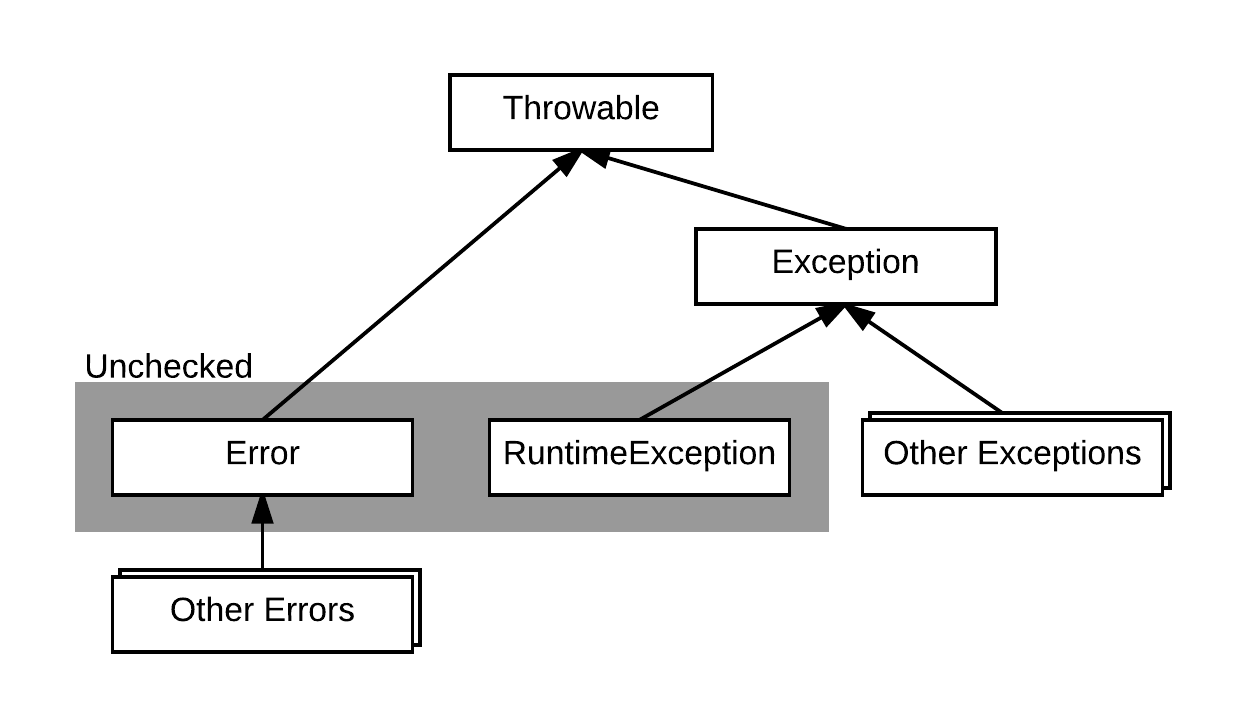
\includegraphics[width=\linewidth, frame]{images/exceptionhierarchy}
\caption{Exception Hierarchy}
\label{fig:exceptions}
\end{figure}

There are two types of \texttt{Exceptions}; checked and unchecked.

\subsubsection{Checked or Uncecked}
Any exception that is a subclass of \texttt{RuntimeException}, a special subclass of \texttt{Exception}, is a so-called "unchecked" exception. All \texttt{Error} subclasses are also unchecked exceptions. There is nothing that the user would reasonable be able to do to overcome them. These exceptions will not generate a compiler error, so that they will not end up cluttering the code unnecessarily. The programmer can completely ignore them, not even plan to catch them at all. \cite{runtimeexception} If we don't catch them, they will bubble up and interrupt the control flow. Eventually the JVM will display the error in the console, and quit.

The checked exceptions are the ones that generate a compiler error if not handled.

When a user of the code is reasonable expected to recover from a exception, we should use checked exceptions. If not, use unchecked exceptions.\cite{runtimeexception}

\subsubsection{Pitfalls}

Using exceptions to control flow is the most common pitfall with error handling. We should not rely on an exception to occur to make decisions on what to do next. Exceptions are just that, exceptions.

In an encapsulated design, though, there are some difficulties. Imagine a method that returns a Dog object, for example. What if the user didn't provide a name for the dog when we instantiate it? Should the code allow creation of a dog without a name? If so, how do we tell the user that the name is required? We can only return a Dog object, so we couldn't replace it with an error object. We could return a Dog object and have it include an error field. The user would be required to check if there is a value in the error field. Or we could put the error in the name field. Another way could be that we have a global error field and if there is an error we store the message there.These are all bad ideas and go against encapsulation and good object-oriented principles. The solution is to throw an exception. The user doesn't get a Dog object back. Instead there is an exception. The user of the method then has to either handle it or ignore it.

These considerations are made at the time of writing the program although, the exceptions occur at the runtime.

\subsubsection{A Specialized Exception}
Usually the Java provided exception classes are sufficient for handling most of the conditions that might arise in a program. There is little need for creating specialized exceptions. Some programmers just like to have all exceptions be their own in a program. When there is an invalid parameter, for example "\@\$\#\%\$*\&" passed into a dogs name, they want to  throw a "\texttt{MyApplicationException}". A better choice would be an existing  \texttt{IllegalArgumentException} instead.

There are some cases, though, when it might be convenient. Imagine a method that wants to return an error code in case of an exception. That code can be used to easily localize the error message shown to the user. 

In order to create our own exception class, we would extend either \texttt{Exception} or \texttt{RuntimeException} (checked or unchecked).
\begin{lstlisting}[language=Java]
public class MyException extends Exception {
// ...
}
\end{lstlisting}

We then would add a field for the error code. 
\begin{lstlisting}[language=Java]
private int errorCode;

public int getErrorCode() {
 return errorCode;
}

public void setErrorCode(int errorCode) {
 this.errorCode = errorCode;
}

@Override
public String getMessage() {
 return super.getMessage() + " (" + errorCode + ")";
}
\end{lstlisting}

We would then override all constructors and let the user pass in the error code. In those constructors we would call the corresponding super constructor and  initialize the error code field. 
\begin{lstlisting}[language=Java]
public MyException(int errorCode) {
 this.errorCode = errorCode;
}

public MyException(Throwable cause, int errorCode) {
 super(cause);
 this.errorCode = errorCode;
}

public MyException(String message, int errorCode) {
 super(message);
 this.errorCode = errorCode;
}

public MyException(String message, Throwable cause, int errorCode) {
 super(message, cause);
 this.errorCode = errorCode;
}
\end{lstlisting}


See Appendix H (MyException.java) on page \pageref{App:AppendixHExeption} for the full source of a sample custom exception.


\subsubsection{Throwing an Exception}
When we have a need to alert about an issue we throw an exception. In order to do that we need to consider two things
\begin{lstlisting}[language=Java, label=lst:throwException]
private void throwCustomException() 
   throws MyException {
 if (someConditionIsTrue) {
   throw new MyException("My message", 404);
  } else {
   System.out.println("Don't throw it...");
  }
}
\end{lstlisting}

We need to add a \texttt{throw} statement where we need to alert about the error, line 4 in listing \ref{lst:throwException}. Also, for checked exceptions, we need to add a \texttt{throws} statement in the method signature (line 2). For unchecked exceptions we don't need to add anything to the method signature.

\subsubsection{Handling an Exception}
When we call a method that throws an exception, we may want to choose to handle it. 

\begin{lstlisting}[language=Java, label=lst:catch]
try {
  throwCustomException();
} catch (MyException e) {
  System.out.println(e.getMessage());
} finally {
  System.out.println("Finally");
}
\end{lstlisting}

We enclose the method that throws an exception in a \texttt{try} block, lines 1-3 of listing \ref{lst:catch}. We have a \texttt{catch} block that handles the exception (lines 3-5). We also have an optional \texttt{finally} block that is executed after the catch block (lines 5-7).

On the other hand, if we choose not to catch an exception, we can propagate it by adding a \texttt{throws} statement in the method signature (line 6 in listing \ref{lst:propagate}).

\begin{lstlisting}[language=Java, label=lst:propagate]
/**
  * We don't catch it, just let it propagate up.
  * If it is a checked exception, someone higher
  * up will eventually have to catch it
  */
private void catchCustomException() throws MyException {
  throwCustomException();
}
\end{lstlisting}

See full listing of the code in Appendix H (ExceptionExample.java)on page \pageref{App:AppendixHExample}.